% Options for packages loaded elsewhere
\PassOptionsToPackage{unicode}{hyperref}
\PassOptionsToPackage{hyphens}{url}
\PassOptionsToPackage{dvipsnames,svgnames,x11names}{xcolor}
%
\documentclass[
doublespace,
  times]{anzsauth}

\usepackage{amsmath,amssymb}
\usepackage{iftex}
\ifPDFTeX
  \usepackage[T1]{fontenc}
  \usepackage[utf8]{inputenc}
  \usepackage{textcomp} % provide euro and other symbols
\else % if luatex or xetex
  \usepackage{unicode-math}
  \defaultfontfeatures{Scale=MatchLowercase}
  \defaultfontfeatures[\rmfamily]{Ligatures=TeX,Scale=1}
\fi
\usepackage{lmodern}
\ifPDFTeX\else  
    % xetex/luatex font selection
\fi
% Use upquote if available, for straight quotes in verbatim environments
\IfFileExists{upquote.sty}{\usepackage{upquote}}{}
\IfFileExists{microtype.sty}{% use microtype if available
  \usepackage[]{microtype}
  \UseMicrotypeSet[protrusion]{basicmath} % disable protrusion for tt fonts
}{}
\makeatletter
\@ifundefined{KOMAClassName}{% if non-KOMA class
  \IfFileExists{parskip.sty}{%
    \usepackage{parskip}
  }{% else
    \setlength{\parindent}{0pt}
    \setlength{\parskip}{6pt plus 2pt minus 1pt}}
}{% if KOMA class
  \KOMAoptions{parskip=half}}
\makeatother
\usepackage{xcolor}
\setlength{\emergencystretch}{3em} % prevent overfull lines
\setcounter{secnumdepth}{5}
% Make \paragraph and \subparagraph free-standing
\makeatletter
\ifx\paragraph\undefined\else
  \let\oldparagraph\paragraph
  \renewcommand{\paragraph}{
    \@ifstar
      \xxxParagraphStar
      \xxxParagraphNoStar
  }
  \newcommand{\xxxParagraphStar}[1]{\oldparagraph*{#1}\mbox{}}
  \newcommand{\xxxParagraphNoStar}[1]{\oldparagraph{#1}\mbox{}}
\fi
\ifx\subparagraph\undefined\else
  \let\oldsubparagraph\subparagraph
  \renewcommand{\subparagraph}{
    \@ifstar
      \xxxSubParagraphStar
      \xxxSubParagraphNoStar
  }
  \newcommand{\xxxSubParagraphStar}[1]{\oldsubparagraph*{#1}\mbox{}}
  \newcommand{\xxxSubParagraphNoStar}[1]{\oldsubparagraph{#1}\mbox{}}
\fi
\makeatother


\providecommand{\tightlist}{%
  \setlength{\itemsep}{0pt}\setlength{\parskip}{0pt}}\usepackage{longtable,booktabs,array}
\usepackage{calc} % for calculating minipage widths
% Correct order of tables after \paragraph or \subparagraph
\usepackage{etoolbox}
\makeatletter
\patchcmd\longtable{\par}{\if@noskipsec\mbox{}\fi\par}{}{}
\makeatother
% Allow footnotes in longtable head/foot
\IfFileExists{footnotehyper.sty}{\usepackage{footnotehyper}}{\usepackage{footnote}}
\makesavenoteenv{longtable}
\usepackage{graphicx}
\makeatletter
\def\maxwidth{\ifdim\Gin@nat@width>\linewidth\linewidth\else\Gin@nat@width\fi}
\def\maxheight{\ifdim\Gin@nat@height>\textheight\textheight\else\Gin@nat@height\fi}
\makeatother
% Scale images if necessary, so that they will not overflow the page
% margins by default, and it is still possible to overwrite the defaults
% using explicit options in \includegraphics[width, height, ...]{}
\setkeys{Gin}{width=\maxwidth,height=\maxheight,keepaspectratio}
% Set default figure placement to htbp
\makeatletter
\def\fps@figure{htbp}
\makeatother

% The following \newcommands are intended for use in the *current*
% document ("protoType"). It is unlikely that authors of papers submitted
% to the Journal will need them.  (Of course if it turns out that you
% do indeed need them, then by all means feel free to make use of them.)
%%%%%%%%%%%%%%%%%%%%%%%%%%%%%%%%%%%%%%%%%%%%%%%%%%%%%%%%%%%%%%%%%%%%%%%%%%%%%%
\usepackage{lipsum}

\newcommand\BibTeX{{\rmfamily B\kern-.05em \textsc{i\kern-.025em b}\kern-.08em
T\kern-.1667em\lower.7ex\hbox{E}\kern-.125emX}}
\newcommand\MiKTeX{{\rmfamily M\kern-.05em \textsc{i\kern-.025em K}\kern-.08em
T\kern-.1667em\lower.7ex\hbox{E}\kern-.125emX}}
\newcommand\PracTeX{{\rmfamily P\kern-.05em \textsc{r\kern-.025em a\kern-.025em
c}\kern-.08em
T\kern-.1667em\lower.7ex\hbox{E}\kern-.125emX}}
%%%%%%%%%%%%%%%%%%%%%%%%%%%%%%%%%%%%%%%%%%%%%%%%%%%%%%%%%%%%%%%%%%%%%%%%%%%%%%


\makeatletter
\@ifpackageloaded{caption}{}{\usepackage{caption}}
\AtBeginDocument{%
\ifdefined\contentsname
  \renewcommand*\contentsname{Table of contents}
\else
  \newcommand\contentsname{Table of contents}
\fi
\ifdefined\listfigurename
  \renewcommand*\listfigurename{List of Figures}
\else
  \newcommand\listfigurename{List of Figures}
\fi
\ifdefined\listtablename
  \renewcommand*\listtablename{List of Tables}
\else
  \newcommand\listtablename{List of Tables}
\fi
\ifdefined\figurename
  \renewcommand*\figurename{Figure}
\else
  \newcommand\figurename{Figure}
\fi
\ifdefined\tablename
  \renewcommand*\tablename{Table}
\else
  \newcommand\tablename{Table}
\fi
}
\@ifpackageloaded{float}{}{\usepackage{float}}
\floatstyle{ruled}
\@ifundefined{c@chapter}{\newfloat{codelisting}{h}{lop}}{\newfloat{codelisting}{h}{lop}[chapter]}
\floatname{codelisting}{Listing}
\newcommand*\listoflistings{\listof{codelisting}{List of Listings}}
\makeatother
\makeatletter
\makeatother
\makeatletter
\@ifpackageloaded{caption}{}{\usepackage{caption}}
\@ifpackageloaded{subcaption}{}{\usepackage{subcaption}}
\makeatother
\ifLuaTeX
  \usepackage{selnolig}  % disable illegal ligatures
\fi
\usepackage[]{natbib}
\bibliographystyle{anzsj}
\usepackage{bookmark}

\IfFileExists{xurl.sty}{\usepackage{xurl}}{} % add URL line breaks if available
\urlstyle{same} % disable monospaced font for URLs
\hypersetup{
  pdftitle={How I rose from the dead in my spare time and so can you},
  pdfauthor={A. J. Specktowsky; Philip K. Dick; Rolf Turner; Emi Tanaka},
  pdfkeywords={anzsauth, bibliographic
references, bibtex, citations, document class, notational
conventions, style guide},
  colorlinks=true,
  linkcolor={blue},
  filecolor={Maroon},
  citecolor={Blue},
  urlcolor={Blue},
  pdfcreator={LaTeX via pandoc}}

\usepackage{moreverb}
\usepackage{url}
\usepackage{grffile}
\usepackage[UKenglish]{isodate}

%%%%%%%%%%%%%%%%%%%%%%%%%%%%%%%%%%%%%%%%%%%%%%%%%%%%%%%%%%%%%%%%%%%%%%%%%%%%%%

% The year in the following may need to be updated!
\def\volumeyear{2024}

% The following command ("obviously") effects line numbering
% of the document.

\usepackage{lineno}
\linenumbers



\runningheads{How I rose from the dead}{A. J. SPECKTOWSKY, PHILIP K.
DICK, ROLF TURNER, EMI TANAKA}

\title{How I rose from the dead in my spare time and so can you}
\usepackage{etoolbox}
\makeatletter
\providecommand{\subtitle}[1]{% add subtitle to \maketitle
  \apptocmd{\@title}{\par {\large #1 \par}}{}{}
}
\makeatother
\subtitle{ANZJS Quarto Template}

\author{
A. J. Specktowsky\addressnum{1},
Philip K. Dick\addressnum{2},
Rolf Turner\addressnum{3} and 
Emi Tanaka
\addressnum{4}\corrauth
}
\affiliation{
School of Hard Knocks, 
School of Design Terrace, 
University of Auckland and 
The Australian National University
}

\address{
\addressnum{1} Department of Redundancy Department, School of Hard
Knocks, Great Falls, MT 54321, USA\break
\addressnum{2} Complaints Division, School of Design Terrace, 30102 East
Rhode Island, Small Planet, Near Betelgeuse\break
\addressnum{3} Department of Statistics, University of Auckland, Private
Bag 92019, Auckland 1142, New Zealand\break
\addressnum{4} Biological Data Science Institute, The Australian
National University, 46 Sullivan's Creek Road, ACT 2600, Australia\\
\hspace*{1ex} Email:    \texttt{emi.tanaka@anu.edu.au}
}


\date{2024}
\begin{document}

\begin{abstract}
This document serves to illustrate some of the main features of the
Quarto based on \LaTeX{} document class \texttt{anzsauth} which authors
are strongly encouraged to use when preparing papers for submission to
the \emph{Australian and New Zealand Journal of Statistics}. The
importance of clarity of exposition as well as a number of issues that
frequently arise in respect of the Journal's standards and conventions
are emphasised. The Journal has precise requirements for the format of
bibliographic references and citations. It is much easier for authors to
conform to these requirements if they use the resources provided by
\BibTeX{} and the \texttt{anzsj} bibliography style (used as default in
this template). Authors are very strongly encouraged to avail themselves
of these resources. The use of \BibTeX{} syntax is illustrated. This
document emphasises a few of the notational conventions that form an
important part of the Journal's stylistic requirements. A great deal
more material about these requirements may be found in the document
``\emph{ANZJS Style Guide for Authors}'' in the file
\href{https://github.com/emitanaka/quarto-anzjs/blob/master/styleGuide.pdf}{\texttt{styleGuide.pdf}}.
\end{abstract}

\keywords{anzsauth; bibliographic
references; bibtex; citations; document class; notational
conventions; style guide}
          
\ack{The author acknowledges that this template is based on the latex
template for Australian and New Zealand Journal of Statistics and
intersperses some text from the original prototype document.
\newline\vspace{1ex}\newline Opinions and attitudes expressed in this
document, which are not explicitly designated as Journal policy, are
those of the author and are \emph{not} necessarily endorsed by the
Journal, its editorial board, its publisher Wiley or by the Australian
Statistical Publishing Association Inc.}

\maketitle

\section{Introduction}\label{sec-intro}

This document show how to use the \texttt{anzjs} Quarto document so as
to be able to produce an article conforming to the Journal's
requirements with a minimum of effort. The correponding template can be
found at

\url{https://github.com/emitanaka/quarto-anzjs}

You are advised to \emph{look carefully} at the source file
\texttt{template.qmd}, and to spend a little while studying the
examples. In particular, read the \emph{comments}.

Papers submitted to the Journal should be \emph{double spaced} and
should have their lines \emph{numbered}. This is important in as much as
it makes it easier for referees and technical editors to indicate where
corrections are required. Double spacing and line numbers are included
by default, but you can disable these by setting \texttt{double-space}
and \texttt{line-numbers} to \texttt{false} in the \texttt{format} field
of the front matter.

A primary requirement that the Journal imposes is that papers must be
written lucidly and in clear and grammatically correct English.
Consequently Section~\ref{sec-clarExpos} is devoted to issues that arise
in respect of good exposition. Other requirements include proper
formatting of the title page. This is done \emph{far} more easily if you
make use of the resources provided by the \texttt{anzsauth} document
class than if you attempt to do the formatting ``by hand''. (See
Section~\ref{sec-titPage}).

The Journal insists that citations should be formed correctly and in
accordance with its conventions. Likewise the list of references must
have the correct structure. Again these requirements are \emph{greatly}
facilitated if you make use of the resources provided (by means of
\BibTeX~and the \texttt{anzsj} bibliography style). These matters are
discussed in Section~\ref{sec-bibRef}.

Although this is \emph{not} handled in an automatic manner, it is
important to adhere to the Journal's notation conventions. Most of the
discussion of notational conventions has been placed in ``\emph{ANZJS}
Style Guide for Authors'' to be found in the file
\href{https://github.com/emitanaka/quarto-anzjs/blob/master/styleGuide.pdf}{\texttt{styleGuide.pdf}}.

Some of the more salient points about notation are dealt with in
Section~\ref{sec-noteConv} in the current document (thus overlapping a
bit with the style guide). Displayed equations and their numbering are
dealt with in Section~\ref{sec-eqnNumb}. In this section some cogent
advice is given about handling arrays of equations. Issues that arise in
respect of the inclusion of figures and tables in a paper are discussed
in Section~\ref{sec-figAndTab}. In Section~\ref{sec-crossref} some
remarks are made, and avuncular advice given, about cross referencing.
Section~\ref{sec-append} presents the Journal's policy about how
appendices should be headed. It also describes the \texttt{Appendix} and
\texttt{uniqueAppendix} environments that are now provided by the
\texttt{anzsauth} document class and that make it easy for you to make
sure that your appendices are headed in the correct manner.
Section~\ref{sec-prepDocs} provides a little bit of advice about
preparing and processing the ``source files'' that underlie the use of
\LaTeX.

It has been pointed out to me that some authors need some guidance as to
what to do with the files \texttt{anzsauth.cls} and \texttt{anzsj.bst}
which come as part of this template.

Various exhortations are reiterated, and some advice about how to make
use of \texttt{template.qmd} is given in Section~\ref{sec-concComm}. In
this last Section you are additionally exhorted to create a \emph{tidy}
Quarto source file.

\section{Clarity of exposition}\label{sec-clarExpos}

Obviously the fundamental consideration in respect of assessing a
paper's quality is its actual content: its correctness and its value in
terms of the advancement of statistical science. Second only to content
is the quality of the exposition of the ideas developed in the paper.
There is little merit in having high quality content if the paper is
written in such a manner that its audience finds it burdensome or even
impossible to read.

The Journal has very exacting standards for the quality of English
expression in the papers it publishes. Authors are expected to think
carefully about the way in which they present material. Ideas should
flow in a logical manner. The connections between successive segments of
the material should be obvious and easy to follow. Succinct and
well-organised examples, kept as uncomplicated as possible, should be
provided to clarify intricate concepts. It is \emph{not} acceptable to
throw down a jumble of ideas in random order and expect the reader to
sort them out. Sufficient explanation should be provided so that any
reasonably well-educated statistician who is willing to expend a
reasonable amount of effort will be able to understand the paper. It is
\emph{not} acceptable for the paper to be comprehensible only to experts
in the relevant field of study (or, worse, only to the authors!).

Diligent attention must be paid to grammar. For instance
\emph{articles}, definite (``the'') and indefinite (``a'' or ``an'')
must be used appropriately. It is not acceptable to omit articles where
they are required, to insert an article where none is required, or to
use a definite article where an indefinite one is required or vice
versa. In a similar vein, agreement in ``number'' between subject and
verb must be carefully maintained. Authors must guard vigilantly against
the use of dangling or misplaced modifiers (an unfortunately common type
of error).

A typical example of a dangling modifier is ``The SE of the correlation
increased in size when changing from 4 to 5 quadrature points. This
sounds as if the SE changed from 4 to 5 quadrature points! A
grammatically correct phrasing might be something like''The SE of the
correlation increased in size when the number of quadrature points was
changed from 4 to 5.'' A typical example of a misplaced modifier is ``A
plot of the residuals from Specktowsky's model shown in Figure 42
indicates the lack of an adequate fit.'' (The \emph{model} is not shown
in Figure 42!) Better would be ``A plot, shown in Figure 42, of the
residuals from Specktowsky's model indicates the lack of an adequate
fit.''

Some might argue that grammatical issues like these ``don't really
matter'' and that ``the meaning is clear''. The meaning is
\emph{sometimes} clear, and sometimes becomes possible to discern only
after readers have expended considerable effort that has been
unnecessarily imposed upon them. Grammatical errors are distracting and
confusing. Reading a paper containing grammatical errors is an
unpleasant experience, and readers will be discouraged from giving a
paper containing such errors the attention that it may otherwise well
deserve. Such errors are an unnecessary encumbrance to a paper and can
be avoided with a modicum of care and diligence. The Journal insists
that such diligence be exercised.

In addition to being written with logical clarity and being free of
grammatical errors, manuscripts should be concise and expressed in a
direct style. Sentences should be kept short; long sentences are hard to
follow and should always be judiciously broken into a number of shorter
sentences. Distracting use of unnecessary technical terms should be
avoided. Do not abbreviate terms unless they are used repeatedly and the
abbreviation is helpful to the reader. Initially use the word in full,
and follow it by the abbreviation in parentheses. Thereafter use the
abbreviation only. Do not abbreviate author names; for example ``Hall
and Heyde (HH)'' must \emph{not} be used.

Care must be taken with the tense of verbs. Use the past tense when
describing something that was done in the past! In particular
simulations should be described in the past tense. For example say ``We
generated 1000 data sets from our parametric model \ldots'' and not ``We
generate 1000 data sets \ldots''. Use the past tense when referring to
results from existing literature. For example, use ``Smith \& Jones
(2007) showed that two plus two equals four'', not ``Smith \& Jones
(2007) show that two plus two equals four''. Use the present tense in
referring to the content of the paper that you are writing: ``In this
paper we show that the convergence rate is \(o_P(n^{-2/3})\).'' (Not
``we showed that''.)

It is the responsibility of the authors to ensure that the use of
English language in the manuscript is of a quality suitable for the
Journal. If you are not absolutely confident that this requirement is
fully satisfied, then have your manuscript checked and \emph{thoroughly}
edited by a suitably qualified person. Such a person (whose first
language should preferably be English) must have superior English
language skills and also be qualified in statistics so as to be able to
assess and correct the expression of statistical ideas.

Failure to ensure an adequate standard of English expression may result
in the paper's being rejected at the Technical Editing stage \emph{even
though} it has previously been assessed by referees and and an associate
editor as being acceptable for the Journal. Referees are experts in the
particular field addressed by a given paper and they assess that paper
for correctness and value of statistical and scientific content. They
rarely read the paper carefully in respect of style and exposition,
assuming that this is not their responsibility. This is why the Journal
explicitly leaves final acceptance to the Technical Editor. The Journal
also reserves the right to modify an accepted paper so as to reduce
inadequacies of exposition. Any such modifications will be discussed
with authors, where feasible.

The Journal's publisher, Wiley, provides a service that can assist
authors with English-language editing. To find out about this service
you may visit:

\url{http://authorservices.wiley.com/bauthor/english_language.asp}

Authors must be aware that there is a \emph{cost} associated with this
service, and this cost must be borne by the author(s) of the paper in
question.

\section{Formatting the title page}\label{sec-titPage}

Do not try to create the list of authors, their affiliations and their
addresses by hand. This is difficult, kludgy and usually leads to
results that are not in keeping with the Journal's requirements (which
eventually makes more work for the typesetters). Look into the
\emph{source} file (\texttt{template.qmd}) that was used to produce this
document. By looking at the structure of this source file, you should be
able to quickly discern the way in which the frontmatter should be used.

Note also that when specifying the abstract, the template produces the
correct heading ``\textbf{Summary}'' as required by the Journal.

By learning to use these resources you will in the long run save a
\emph{great} deal of time and dramatically reduce the effort that you
expend.

\subsection{Bibliographic references}\label{sec-bibRef}

\subsection{The Journal's citation rules}\label{sec-citeRules}

The Journal (for the sake of consistency; see
Section~\ref{sec-noteConv}) imposes a number of strict rules or
conventions on the way that citations are formed. Authors \emph{must}
follow these conventions. Just as you are advised not to format the
title page ``by hand'', you are strongly encouraged not to produce your
citations and your list of references in an ad hoc one-by-one manner.
Instead use the (very well designed) tools that are available for the
purpose. That is, make use of \BibTeX~and the \texttt{anzsj}
bibliography style (see Section~\ref{sec-useBib}). If you do so, then
(most of) the Journal's required conventions will be followed
automatically, thereby saving you a great deal of work and a great many
headaches.

If you insist on ``doing things your own way'', then you must \emph{read
carefully} the relevant section of ``\emph{ANZJS Style Guide for
Authors}'' and carefully follow the specifications given.

A rule that \BibTeX~and the \texttt{anzsj} bibliography style will
\emph{not} automatically handle for you is that the names of journals
appearing in the reference list must \emph{not be} abbreviated. This is
a

\begin{center}
{\large \textbf{CHANGE or REVERSAL}}
\end{center}

of Journal policy from what it has been in the past. (One might be
inclined to say that it is an ``about face'' or retreat, or climb-down.)
If you have struggled to dutifully make your references accord with the
previous policy that demanded that journal names be abbreviated in
accordance with ``standard abbreviations'' and have arduously combed the
web to find out just what these standard abbreviations are \ldots~well,
I can only apologise. You are however owed some explanation:

The Editorial Board were unanimously of the opinion that the policy of
demanding abbreviated Journal names was probably adopted in the dim
distant past to save time for typesetters, and has little function in
today's circumstance. The only actual benefit of this policy is that
there is a tiny space saving, and this tiny benefit comes at the cost of
unnecessarily adding tedious work to authors' responsibilities. It also
has the disadvantage of making our papers less accessible to readers,
especially non-statisticians/mathematicians. Some readers may know that
\emph{Stat. Neerl.} is \emph{Statistica Neerlandica}, but many will not.
The change in policy is one small step toward making statistics research
more user-friendly.

Consequently \emph{please} do not abbreviate journal names. At all.
Ever. Please \emph{consistently} give journals their full title. Again I
apologise (on behalf of the Editorial Board) if this causes you
inconvenience and results in your having wasted (substantial) time and
effort.

Another rule that cannot be automatically handled is that reference may
not be made to a paper ``submitted for publication'' or to a ``personal
communication''. The essential criterion for inclusion in the reference
list is that any such reference must be obtainable by a reader: thus a
Technical Report is OK and a paper accepted for publication is OK. You
may, if you wish, put into the text a kind of acknowledgement of the
form ``It was pointed out to me by Fred Nurk (\emph{pers. comm.}) that
Bayesian statistics is a load of dingoes' kidneys.'' However such
references must \emph{not} be listed in your bibliography.

Likewise references to unpublished data may be cited in the text
(e.g.~``I. Poobah, unpublished data, 2000)'' but must not appear in the
list of references. Otherwise all citations mentioned in the text,
tables or figures must be listed in the reference list. A work must
\emph{not} appear in the reference list \emph{unless} it is cited in the
text.

\section{\texorpdfstring{Using \BibTeX~}{Using ~}}\label{sec-useBib}

Authors are \textbf{\emph{STRONGLY}} encouraged to make use of the
resources provided by \BibTeX~in preparing their lists of references and
in citing these references in their documents. This is easy to do and
helps to make sure that the reference list and citation conventions
conform to the Journal's requirements. The Journal has its own
``bibliographic style'' (``\texttt{anzsj}'') which is based upon the
\texttt{natbib} package.

To use \BibTeX~you need to do the following:

\begin{enumerate}
\def\labelenumi{\arabic{enumi}.}
\tightlist
\item
  Prepare a ``bibliographic information'' (\texttt{*.bib}) file
  containing appropriately structured information about all of the
  references that you will cite in your document. Note that this file
  can contain information about references that you \emph{do not cite}
  in your document. Only those references cited will appear in the list
  of references. This allows you to prepare a single bibliographic
  information file that can be used for multiple papers with overlapping
  but not identical reference lists. Of course when submitting a paper
  you may wish to upload only a cut-down \texttt{*.bib} file that
  contains only the relevant references (rather than a very large
  bibliographic information file with a plethora of irrelevant entries).
  \newline The way that the information in your bibliographic
  information file should be structured is illustrated by the example
  file \texttt{bibliography.bib} that accompanies the document that you
  are currently reading. Imitating the entries in this example file
  should allow you to create just about any references you need to use.
  Note that some rather off-beat entries in \texttt{bibliography.bib}
  are not cited in this paper and hence do not appear in the
  bibliography. This is in accordance with the rule that \emph{only}
  literature which is actually cited may appear in the list of
  references. Four of these entries are referred to in commented-out
  \texttt{nocite} in the front matter at the start of the source file
  \texttt{template.qmd}. If you want to see what bibliography entries
  these items would produce, just un-comment the \texttt{nocite} lines
  and then compile \texttt{template.qmd}. More information about the
  structure of \texttt{*.bib} files may be found in
  \citet{MittelbachGoossens2004}. There are also many resources to be
  found on the web by doing a Google\texttrademark\\
  search on ``\texttt{bibtex}''.
\end{enumerate}

At the start of your Quarto document, add
\texttt{bibliography:\ xxx.bib} where ``\texttt{xxx.bib}'' refers to the
name of your bibliographic information file.

\subsection{Citing references}\label{sec-citRef}

Cite references by using \texttt{@ref-id} and variants thereof. Some
discussion of the possible variants is to be found in
Section~\ref{sec-citeVar}. The
\texttt{ref-id\textasciigrave{}\textasciigrave{}\ represents\ the\ identifier\ for\ the\ item\ being\ cited.\ \ If\ you\ (sensibly)\ use\ \textbackslash{}BibTeX,\ the\ identifier\ is\ provided\ in\ the\ first\ line\ of\ the\ bibliographic\ information\ about\ the\ item\ being\ cited.\ \ For\ example\ \_The\_\ \textbackslash{}LaTeX\textbackslash{}\ \_Companion\_\ referred\ to\ above\ was\ cited\ in\ this\ document\ via}\citet{MittelbachGoossens2004}\texttt{.\ \ The\ relevant\ item\ in}bibliography.bib`
begins

\begin{verbatim}
    @book{MittelbachGoossens2004,
\end{verbatim}

If you do not use \BibTeX, then the identifier is given as the
``\texttt{cite\_key}'' for the appropriate item in the list of
references following
\texttt{\textbackslash{}begin\{thebibliography\}\{...\}} line in your
\LaTeX~document.

The way that the identifier is formed is fairly arbitrary; construct
identifiers in your bibliographic information file in whatever way suits
your fancy. My personal paradigm is to construct identifiers from the
author's name (or authors' names) followed by the year as in the example
given above. If there are more than two authors I just use the first
author's name followed by ``EtAl'' and the year. E.g. for an article by
Fred Nurk, Melvin Mingdinkler and Hoo Hee, published in 1984, I use the
identifier \texttt{NurkEtAl1984}. I emphasise that this is just my
personal convention that I have found useful; you are under no
obligation to follow it.

\subsection{Variants of the basic citation command}\label{sec-citeVar}

In addition to the ``usual'' citation command ``\texttt{@ref-id}'' there
are a number of alternative citation commands that can be used to create
special punctuation structures in particular circumstances. See more on
the Quarto documentation site
\href{https://quarto.org/docs/authoring/citations.html\#sec-citations}{here}.

Yet another variant of \texttt{@ref-id} is \texttt{{[}@ref-id{]}} which
encloses the whole citation, rather than just the year, in parentheses.
E.g. ``Some authors prefer the hack \citep{Cook1966}, others the hew
\citep{Moore1967}, and still others opt for a combination
\citep{CookMoore1968}.''

\subsection{Notational conventions}\label{sec-noteConv}

It may seem dogmatic, but the Journal has some strict rules about
notational conventions that must be followed. The reason for these rules
is simply \emph{consistency}. One and only one convention must be
followed, otherwise the result is a visually unpleasant hodge-podge.
Which convention is chosen does not usually matter very much, but a
single one must be chosen and used consistently. The choice is made by
the Journal; authors must follow it.

A few of the more important examples of these conventions are listed
below. Many others are given in the document ``\emph{ANZJS} Style Guide
for Authors'' as mentioned in Section~\ref{sec-intro}.

\begin{enumerate}
\def\labelenumi{\arabic{enumi}.}
\tightlist
\item
  The transpose operator: This must be represented as a sans-serif
  \(\top\), which is most easily rendered in \LaTeX\\
  by \texttt{\textbackslash{}top}.
\item
  The symbols ``\(\forall\)'' and \(\exists\): Do \emph{not} use them!
  Use \emph{words} --- ``for each'' or ``for all'' and ``there
  exist(s)''.
\item
  Random and non-random quantities: (Scalar) random variables should
  generally be denoted by upper case letters such as \(X\) or \(Y\).
  Non-random quantities should be denoted by lower case letters. An
  observed value of \(Y\) would be denoted by \(y\).
\item
  Vectors and matrices: Vectors quantities should be indicated by bold
  face font, e.g.~\(\by\). Vectors of observations should be presented
  as (boldface) lower case letters (such as the \(\by\) example just
  given) whereas vectors of random variables should be presented as bold
  face upper case letters: \(\bY\). Matrices should also be presented as
  bold face upper case letters: \(\bM\). To help you to adhere to these
  conventions there are now commands \texttt{\textbackslash{}bx},
  \texttt{\textbackslash{}by}, \texttt{\textbackslash{}bX},
  \texttt{\textbackslash{}bY} and \texttt{\textbackslash{}bM} defined in
  the \texttt{anzsauth} document class that produce \(\bx\), \(\by\),
  \(\bX\), \(\bY\) and \(\bM\) respectively. To get other bold face
  letters, have a look at the file \texttt{anzsauth.cls} and imitate the
  construction of the foregoing commands.
\item
  Expectation: Use ``E'' (upright Roman font) for the expectation
  operator, and enclose the argument of this operator in
  \emph{parentheses} as in \(\E(X)\). \label{op:expect}
\item
  Variance, covariance and correlation: Likewise use ``var'', ``cov''
  and ``cor'' (ordinary Roman font, all lower case) for the variance,
  covariance and correlation operators, as in \(\var(X)\), \(\cov(X,Y)\)
  and \(\cor(X,Y)\). \label{op:var}
\item
  Probability: Use ``\(\Pr\)'' for the probability function, and enclose
  the argument of this function in \emph{parentheses} as in \(\Pr(A)\).
  The probability function is best rendered in \LaTeX~by using
  \texttt{\textbackslash{}Pr}.
\item
  Do not begin sentences with symbols (mathematical or otherwise). A
  sentence \emph{must} begin with a \emph{word} that can be capitalised.
  For example, instead of ``\(\Phi(x)\) is a cumulative distribution
  function \ldots'', use ``The function \(\Phi(x)\) is a cumulative
  distribution function \ldots''.
\end{enumerate}

To help you adhere (effortlessly!) to the conventions specified in items
\ref{op:expect} and \ref{op:var} there are now commands
\texttt{\textbackslash{}E}, \texttt{\textbackslash{}var},
\texttt{\textbackslash{}cov} and \texttt{\textbackslash{}cor} defined in
the \texttt{anzsauth} document class. This is effected by means of the
\texttt{\textbackslash{}newcommand\{\}} facility provided by \LaTeX.
These commands produce the required form of the expectation operator and
the variance, covariance and correlation operators.

Other notational structures can be created in a similar manner. Look
into the \texttt{anzsauth.cls} document class file; it's a plain text
file; it won't bite! By imitating \texttt{\textbackslash{}E},
\texttt{\textbackslash{}var}, \texttt{\textbackslash{}cov},
\texttt{\textbackslash{}cor} and other examples, you will be able to
construct a convenient ``shorthand'' that will allow you to produce
notation conforming to the Journal's requirements using a minimal number
of keystrokes.

\subsection{Equation numbering}\label{sec-eqnNumb}

An equation should be given a number \textbf{\emph{ONLY IF}} if it is
referred to elsewhere in the paper. Use \texttt{\$\$\ ...\ \$\$} to
display an equation \emph{without} a number. You can use
\texttt{\textbackslash{}begin\{align*\}\ ...\ \textbackslash{}end\{align*\}}
for equations that span mulitple lines. You will need to have the
package \texttt{amsmath} loaded in order to have access to the
\texttt{align*} (and the \texttt{align} and \texttt{split} --- see
below) environments. Examples:

\[\Pr(K = k) = \binom{n}{k} p^k (1-p)^{n-k}\]

and \begin{align*}
P_0(x) &= 1 \\
P_1(x) &= x \\
P_2(x) &= (3x^2 - 1)/2 \\
P_3(x) &= (5x^3 - 3x)/2 \\
       & \ldots \\
P_{n+1}(x) &= ((2n+1)xP_n(x) - nP_{n-1}(x))/(n+1)
\end{align*} Use \texttt{\$\$\ ...\ \$\$} followed by an equation id,
e.g.~\texttt{\{\#eq-example\}} to display an equation \emph{with} a
number. You can use
\texttt{\textbackslash{}begin\{eqnarray\}\ ...\ \textbackslash{}end\{eqnarray\}}
to display an array of equations with numbers, but as for un-numbered
arrays of equations it is better to use
\texttt{\textbackslash{}begin\{align\}\ ...\ \textbackslash{}end\{align\}}.
Very often you will wish to have only one number associated with an
array of equations. To suppress equation numbers you can use the
\texttt{\textbackslash{}nonumber} command with \texttt{align}, but you
get a sexier result if you use \texttt{split} inside an equation
environment. Examples: \begin{equation}\phantomsection\label{eq-GNZ}{
\E \left (\sum_i h(x_i,\bX \setminus \{x_i\}) \right )
= \E \left ( \int_W h(u,\bX) \lambda(u,\bX) \; du \right )
}\end{equation} and

\begin{equation}\phantomsection\label{eq-gammaMM}{\begin{split}
\alpha \beta &= \bar{x} \\
\alpha \beta^2 &= s^2 \;\; .
\end{split}
}\end{equation}

Note how the label (i.e.~``(\ref{eq-gammaMM})'') is vertically centred
with respect to the array of equations. See the \LaTeX\\
source for the foregoing example in the file \texttt{template.qmd} for
guidance as to how all this is done.

Displayed equations which \emph{are} numbered should be numbered
consecutively (1), (2), \ldots, throughout the paper, including in the
appendices if any. (I.e. they should \emph{not} be numbered ``within
sections''.) The required behaviour is the default in \LaTeX. As long as
you do not take any overt action to mess it up, you will get the
appropriate style in your document.

\subsection{Figures and tables}\label{sec-figAndTab}

Figures and tables often cause problems with the processing of papers.
Here are a few comments on the preparation and presentation of such
displays, with an example of each type. Of course the ``content'' of
these examples is just flippant, frivolous nonsense, as my examples
usually are. (These examples are meant to be humorous; as I indicated
previously, whether you find them funny depends on your sense of
humour.)

It can be a major annoyance if authors supply each panel of a
multi-panel figure as a separate figure file. When this is done, authors
usually proceed by arranging the panels, within an array that
constitutes a single figure, by juxtaposing the commands used to input
the figures in an appropriate manner and interleaving appropriate line
breaks. Although this is all do-able, and may lead eventually to a
visually acceptable figure, it makes extra work both for the author and
for the typesetters. It may also add a substantial amount of tedious
work to the procedure of uploading the final version of the paper to
ScholarOne if you upload the figures individually (rather than in a zip
archive, this last now being acceptable to ScholarOne).

It is much better to create a multi-panel figure in a single figure
file, using appropriate graphics techniques.

\begin{figure}

\centering{

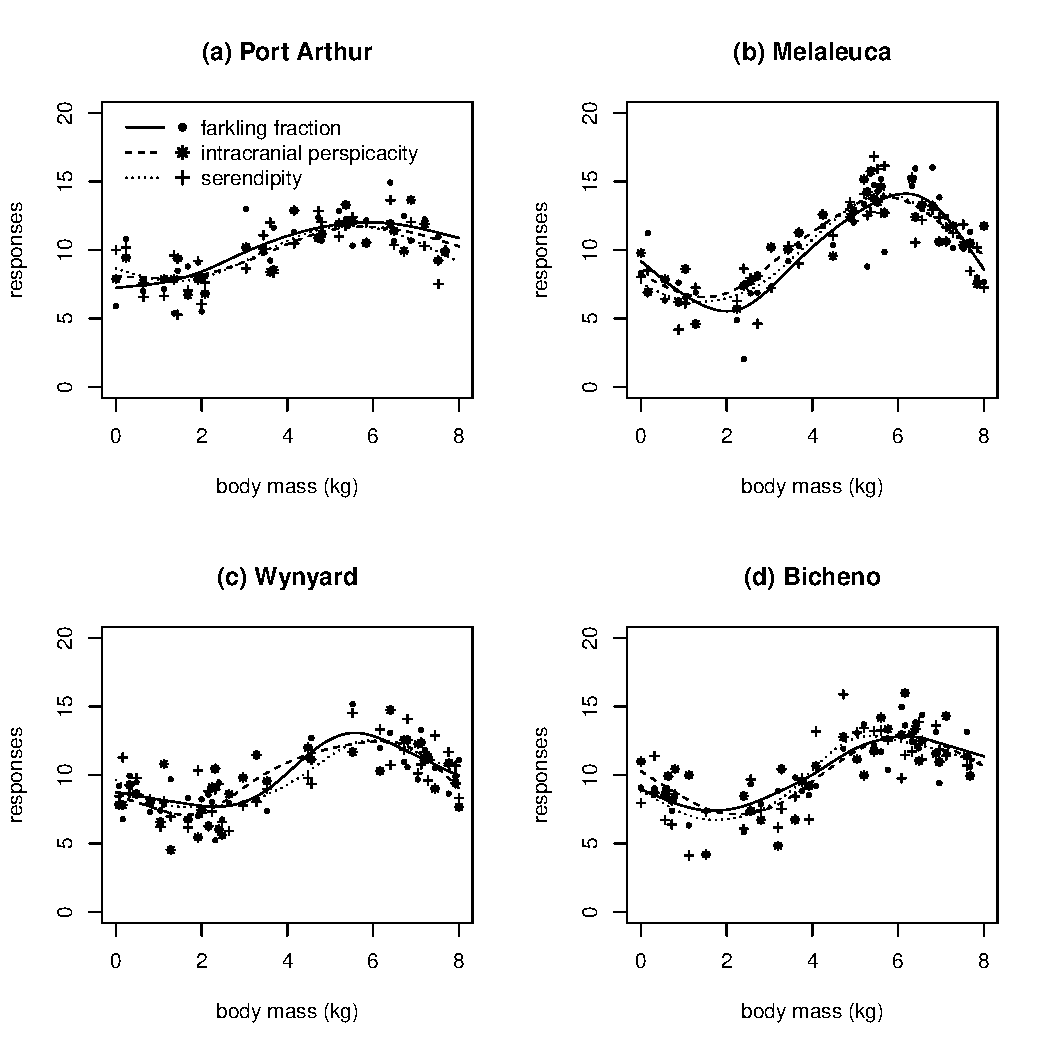
\includegraphics{ltdbFigure.pdf}

}

\caption{\label{fig-ltdb}Characteristics of the Lesser Tasmanian Drop
Bear (farkling fraction, intracranial perspicacity and serendipity all
in furlongs per fortnight) plotted against body mass (kilograms). The
observations were made on samples obtained at four locations in
Tasmania. Plotted points represent the raw observed values; plotted
lines represent non-parametric fits to the raw data.}

\end{figure}%

Another important issue is making sure that line types and plotting
symbols are \emph{distinguishable} in black and white. Figures appear in
the print version of the Journal in black and white \emph{only}, unless
authors specifically request that some or all of the figures appear in
colour and are \emph{willing to pay a charge} to cover the extra costs
that are incurred in printing colour figures. So unless you wish to pay
this charge --- roughly speaking \$350 USD per figure --- you should
prepare your figures in black and white, and do this from the very
start. (Figures that are prepared in colour and then converted to black
and white in the printing process usually look awful! Consequently the
Journal does not countenance this practice.) In particular, lines in
different categories should be distinguished by \emph{line type} ---
solid, dashed, dotted \ldots, and not by colour. A modest example is
given in Figure~\ref{fig-ltdb}. Sometimes it is useful, or perhaps even
necessary, to distinguish categories by means of line \emph{thickness}
but proceeding in this way requires a great deal of care.

Note that colour figures can appear in the online version of the paper
for \emph{free}! However care must be taken, since \emph{only one}
version of the text of the paper is produced. Consequently the online
colour figures, and captions and references to figures in the text, must
be structured in such a way as to make sense both to readers of the
black-and-white (print) version and the colour (online) version. See
\texttt{styleGuide.pdf}, Section 5.1, for a bit more detail.

A common error in respect of tables is making them overly elaborate.
Remember that the purpose of a table is to convey information! If a
table is excessively complex, the reader's eyes will glaze over and he
or she will skip the table, resulting in no information at all being
conveyed. In particular, if a table is too wide to fit on a page and has
to be rotated 90\(^\circ\) in order to be displayed, then you are trying
to put an excessive amount of information into a single table. The
Journal will henceforth \emph{insist} that tables fit vertically onto a
single page. If your paper contains tables that do not satisfy this
condition then you will be required to re-design your table accordingly.
Possibilities for effecting the re-design include eliminating some of
the ``information'', splitting the table into two or more smaller tables
and putting all or part of the table into the online supplementary
material. An example of a reasonably perspicuous table is given in
Table~\ref{tbl-ltdb}.

\begin{longtable}[]{@{}
  >{\raggedright\arraybackslash}p{(\columnwidth - 8\tabcolsep) * \real{0.1594}}
  >{\raggedleft\arraybackslash}p{(\columnwidth - 8\tabcolsep) * \real{0.1884}}
  >{\raggedleft\arraybackslash}p{(\columnwidth - 8\tabcolsep) * \real{0.2319}}
  >{\raggedleft\arraybackslash}p{(\columnwidth - 8\tabcolsep) * \real{0.2319}}
  >{\raggedleft\arraybackslash}p{(\columnwidth - 8\tabcolsep) * \real{0.1884}}@{}}
\caption{A load of dingoes' kidneys in respect of characteristics of the
Lesser Tasmanian Drop Bear. Standard deviations are given in parentheses
after the mean values.}\label{tbl-ltdb}\tabularnewline
\toprule\noalign{}
\begin{minipage}[b]{\linewidth}\raggedright
Location
\end{minipage} & \begin{minipage}[b]{\linewidth}\raggedleft
Body mass (kg.)
\end{minipage} & \begin{minipage}[b]{\linewidth}\raggedleft
Farkling fraction
\end{minipage} & \begin{minipage}[b]{\linewidth}\raggedleft
Intracranial perspicacity
\end{minipage} & \begin{minipage}[b]{\linewidth}\raggedleft
Serendipity
\end{minipage} \\
\midrule\noalign{}
\endfirsthead
\toprule\noalign{}
\begin{minipage}[b]{\linewidth}\raggedright
Location
\end{minipage} & \begin{minipage}[b]{\linewidth}\raggedleft
Body mass (kg.)
\end{minipage} & \begin{minipage}[b]{\linewidth}\raggedleft
Farkling fraction
\end{minipage} & \begin{minipage}[b]{\linewidth}\raggedleft
Intracranial perspicacity
\end{minipage} & \begin{minipage}[b]{\linewidth}\raggedleft
Serendipity
\end{minipage} \\
\midrule\noalign{}
\endhead
\bottomrule\noalign{}
\endlastfoot
Port Arthur & 3.95 ( 2.40) & 10.14 ( 2.43) & 9.91 ( 1.99) & 9.81 (
2.24) \\
Melaleuca & 4.55 ( 2.41) & 10.48 ( 3.51) & 10.83 ( 2.94) & 10.54 (
3.30) \\
Wynyard & 3.87 ( 2.70) & 9.51 ( 2.20) & 9.40 ( 2.44) & 9.50 ( 2.23) \\
Bicheno & 4.16 ( 2.41) & 10.46 ( 2.44) & 10.44 ( 2.64) & 10.20 (
2.86) \\
\end{longtable}

As stated in the ``\emph{ANZJS} Style Guide for Authors'' captions for
tables and figures should be left-justified and not centred unless the
text of the caption fits on a single line. However one-line captions
should be centred. For instance if the caption of Table~\ref{tbl-ltdb}
were simply ``Dingoes' kidneys'', then centring would be preferable.
When the \texttt{anzsauth} document class is used, captions are
automatically centred if the caption fits on a single line. (Note that
the document class file \texttt{anzsauth.cls} has recently --- as of
\printdateTeX{2016/11/06} --- been adjusted to make table captions more
similar in appearance to figure captions. Because of this adjustment,
the centring of one-line table captions is now automatic whereas,
previously, overt measures were required.)

A table or figure that appears in the paper \emph{must} be referred to
in the text, even if only very briefly. That is, there must at the very
least be something like ``see Figure\textasciitilde17''. If there is no
such reference, then the corresponding table or figure must not be
included in the paper.

\section{Cross referencing}\label{sec-crossref}

A facility provided by \LaTeX~that tends to be underused in submissions
to the Journal is automated cross-referencing as provided by the
\texttt{@...} and \texttt{\#} commands. See Quarto documentation for
more on this! It is highly recommended that you learn to make use of
these. They make it much easier to keep cross-references correct when
you revise a paper. It seems to me to be a good idea to give a label to
each section and subsection, as you are composing it, even if you are
not sure you will be referring to it in other sections. (There is no
\emph{harm} in inserting a label.) If you assign labels to sections then
you can easily invite the reader to ``see Section~\ref{sec-figAndTab}''
(as I am about to do below!). Likewise it is a good idea to give each
figure and table (see Section~\ref{sec-figAndTab}) a label so as to be
able to refer to it via the \texttt{\textbackslash{}ref\{...\}} command.

Only displayed equations that are \emph{actually referred to} should be
numbered (see Section~\ref{sec-eqnNumb}). If the equation \emph{is}
referred to, then of course you should give it a label so that you
\emph{can} refer to it easily.

My personal practice is to label sections and subsections with labels of
the form \texttt{sec-string}, e.g.~``\texttt{\#sec-intro}''. Similarly I
form such labels for figures and tables as \texttt{fig-string} or
\texttt{tbl-string} (e.g. \texttt{@fig-ltdb} or \texttt{@tbl-ltdb}) and
labels for equations as \texttt{@eq-string} (e.g.~\texttt{\#eq-GNZ}). I
find this practice convenient, but you are of course under no obligation
to follow it.

A practice that I have often seen and that I think should \emph{not} be
indulged in, is to use labels such as ``\texttt{Figure1}''. There is
\emph{not necessarily} any harm in this, but to a large extent such a
practice defeats the purpose of using dynamic labels. If you decide to
change the order in which figures appear in your paper, then the label
``\texttt{Figure1}'' will probably no longer be appropriate. At best you
will confuse yourself, and you run a serious risk of getting labels
wrong. Use labels that refer to \emph{content} (in a terse manner, of
course) and let \LaTeX~handle the assignment of numbers! If you insist
on using labels like unto ``\texttt{Figure1}'', then take great care to
make sure that the result is correct.

\section{Appendices}\label{sec-append}

Journal policy is that if there is a single appendix to your document it
should be headed simply `\textbf{Appendix}' (i.e.~there should be no
other text in the header and no number). If the document has more than
one appendix these should be headed \textbf{Appendix} I,
\textbf{Appendix II}, \ldots (i.e.~there should be no other text in the
headers, and numbering should be in upper case Roman numerals).

Do \emph{not} use the `native' \LaTeX~command
\texttt{\textbackslash{}appendix}!.

To make it easy to supply appendix headers in the appropriate style, the
\texttt{anzsauth} document class provides two new environments:
\texttt{uniqueAppendix} and \texttt{Appendix}. Use the former if your
document has a single appendix, and the latter if it has more than one.
The use of the \texttt{Appendix} environment is illustrated by means of
the dummy appendices Appendix\textasciitilde{}\ref{app:mung},
Appendix\textasciitilde{}\ref{app:gorp} and
Appendix\textasciitilde{}\ref{app:zephod}. These mostly consist of
``Lorem ipsum'' nonsense Latin and are to be found at the end of this
document that you are currently reading.

The \texttt{\textbackslash{}label\{\}} and
\texttt{\textbackslash{}ref\{\}} commands work with appendices (when
there are multiple appendices). Just put a label within the relevant
\texttt{Appendix} environment and then refer to that appendix with
constructions like
``\texttt{See\ Appendix\textasciitilde{}\textbackslash{}ref\{lll\}}'',
where ``\texttt{lll}'' is the label that you have assigned to the
Appendix in question. Obviously if you have a unique appendix you can
just say (e.g.) ``See the Appendix \ldots'' and there is no need for
labelling.

In order to illustrate the use of \texttt{uniqueAppendix} I had to
invoke it even though there are actually multiple appendices (four in
all) in this document. Don't \emph{you} do that! Do as I say, not as I
do!

The text constituting the illustration of \texttt{uniqueAppendix}
consists of a recapitulation of the foregoing note.

\section{\texorpdfstring{Preparing \LaTeX~and
\BibTeX~documents}{Preparing ~and ~documents}}\label{sec-prepDocs}

\subsection{\texorpdfstring{Editing \LaTeX~source
files}{Editing ~source files}}\label{sec-editors}

There are a number of approaches to preparing your \texttt{*.tex} and
\texttt{*.bib} files. A primary consideration is that you should use
either a general \textbf{text editor}, or a specialised \LaTeX{} editor
for this task. Do \emph{not} use a word-processing program as an editor.
Using a word-processor introduces a plethora of spurious non-printing
characters which will completely mess things up and in all likelihood
cause the universe to come to an end.

Good text editors include \texttt{vi} or \texttt{vim}, \texttt{emacs},
\texttt{gedit}, \texttt{pico}, \texttt{Crimson},
\texttt{Notepad++},\textasciitilde{}\ldots~. Good editors will have
support for editing of \LaTeX{} such as syntax highlighting and code
completion. The Windows\texttrademark~editors \texttt{Notepad} and
\texttt{Wordpad} are distinctly inferior in this respect.

Among a number of possible specialised \LaTeX{} editors, one that has
been highly recommended to me by several reliable sources is
\texttt{TeXstudio}. This is an open-source, multi-platform,
fully-featured editor for \LaTeX{}. It allows for easy processing of
documents, has support for inclusion of a vast range of characters,
provides auto-completion of \LaTeX{} commands, has a built-in pdf viewer
and a number of other helpful facilities. Other similar programs are
\texttt{Texmaker} and (Windows\texttrademark~only) \texttt{WinEdt}.

Users of Windows\texttrademark~will almost surely make use of \LaTeX~via
\MiKTeX. This is free open source software, and is readily available and
easy to install.

The integrated development environment (IDE) \texttt{proTeXt} is
described as being ``an easy-to-install \TeX{} distribution for
Windows\texttrademark, based on \texttt{MiKTeX}'', ``which adds the
\texttt{TeXstudio} front end to MiKTeX''. Some authors may find it
helpful.

\section{Concluding comments}\label{sec-concComm}

This document contains guidance on how to prepare a paper for submission
to \emph{ANZJS} by making use of the `anzsauth\} document class for
\LaTeX. You will find that by making use of this document class and
following the advice that is provided in the foregoing material, you
will be able to produce a paper that meets the Journal's requirements
and that requires much less revision and adjustment than it otherwise
might, thus speeding up the publication process considerably.

This document also emphasises the importance of good exposition and
correct use of the English language. The Journal has very high, and
strictly enforced, standards in this regard. Please pay close attention
to this requirement and give careful thought to the way in which you
express yourself. Doing so will, again, speed up the publication process
for you.

The accompanying file \texttt{template.qmd} forms a template for
\LaTeX~source files for papers that are to be submitted to the Journal.
When preparing your own \LaTeX~source file, you should imitate the
structure of the template closely. You may find that an effective way to
proceed is to edit the template, \emph{mutatis mutandis}, replacing
authors' names, the title of the paper, the abstract (summary) and the
actual content as is appropriate. \emph{Please} remove extraneous bits
and pieces from the prototype file when converting it into your own
paper. Don't leave material that is relevant only to the prototype
(e.g.~comments advising you how to format your paper) lying around. Tidy
up! This makes processing your paper for publication much easier (and
quicker!). In respect of tidyness I draw your attention to the last
paragraph of this section (keep the typescript in your source file
tidy!).

With regard to removing extraneous material, it turns out to be
expedient for me to mention that the disclaimer at the end of the
footnotes on the title page of this document should \emph{not} be
included when you adapt the prototype source file to your own uses. That
disclaimer applies to \emph{this paper}, i.e.~``\textbf{How I rose from
the dead in my spare time and so can you}''. The Journal does \emph{not}
require you to include such a disclaimer in \emph{your} paper, nor
should you do so.

Although it is not necessary to prepare the initial submission using the
\texttt{anzsauth} document class, it is very important that the final
version that you submit (after provisional acceptance of your paper)
should conform to the Journal's requirements. This is much more likely
to be the case if you use the \texttt{anzsauth} document class. It is
likely to be less work for you if you make use of this document class
and of the template from the outset, if this is at all possible. Note
that it \emph{is} necessary for the initial submission to be double
spaced and to be line-numbered. These requirements are greatly
facilitated by using the required document class.

It is often the case that the Technical Editor will wish to make some
minor (or sometimes major!) adjustments to the \LaTeX~source file that
you provide, before putting the paper into production. This saves having
to send the paper back to authors, yet one more time, to get these
adjustments made. The process of making these adjustments is a
\emph{whole lot} easier if the source file is constructed in a tidy and
comprehensible manner. Use appropriate line breaks (keeping lines to a
length of, e.g., at most 80 characters) and ensure that there is
appropriate \emph{spacing} between mathematical constructions. Do not
embed \LaTeX~commands to produce displayed equations in on-running lines
of text. All of this will have of course absolutely no impact on the
\emph{output} file produced by compiling the \LaTeX~source, but it
simplifies the process of modifying and adjusting this source by orders
of magnitude.

\begin{Appendix}
\label{app:mung}

This is an appendix. \lipsum[1]

\end{Appendix}

\begin{Appendix}
\label{app:gorp}

This is another appendix. \lipsum[2]

\end{Appendix}

\begin{Appendix}
\label{app:zephod}
\begin{center}
Zephod Beeblebrox
\end{center}


\emph{This} appendix was written by Zephod Beeblebrox, but he didn't
actually have anything to say. \lipsum[3]

\end{Appendix}

\begin{uniqueAppendix}

This is what you should get if you had only \emph{one} appendix.
Since this document has several appendices (four, actually) the
use of the \texttt{uniqueAppendix} environment is completely
inappropriate here.  It is included for illustrative purposes
only.  I needed to illustrate syntax to be used both for multiple
and unique appendices, but obviously one cannot have a single
document in which there is a unique appendix and in which there are
multiple appendices!  (That would violate the, uh, law of small
numbers. \verb! :-) !)  Consequently I was forced to include an
inappropriate example of the use of \texttt{uniqueAppendix}.

I reiterate:  Use the \texttt{uniqueAppendix} environment if there is
only one appendix to your document.  Use the \texttt{Appendix}
environment if there are two or more appendices to your document.
\end{uniqueAppendix}


  \bibliography{bibliography.bib}


\end{document}
